\graphicspath{{img/compact_objects/}}



\chapter{A Primer on Compact Objects}
\label{chapter:compactobjects}

% \begin{synopsis}
% Introduce COs, formation, structure etc...  
% \end{synopsis}
%%%%%%%%%%%%%%%%%%%%%%%%%%%%%%%%%%%%%
%%%%%%%%%%%%%%%%%%%%%%%%%%%%%%%%%%%%%
%%%%%%%%%%%%%%%%%%%%%%%%%%%%%%%%%%%%%

Within the cores of stars, there exists a delicate balance between the gravitational forces pulling the matter inward, and the outward pressure generated by the thermonuclear fusion of light elements. This process begins as hydrogen is fused to form helium. Eventually, the hydrogen is depleted, allowing gravity to temporarily overcome the outward pressure, leading to the core to begin contracting. As this occurs, the gravitational potential energy is converted to thermal energy and the core eventually becomes hot enough to facilitate helium burning. 

This cycle can continue as heavier and heavier elements are formed within the ever-increasingly hot stellar core. Lighter stars cannot reach the temperatures required to fuse light elements such as helium and carbon. If the star is heavy enough, iron will eventually be formed from the burning of silicon. As the fusion of iron nuclei is an endothermic process, it will not occur spontaneously, ending the cycle in heavy stars. Without a fuel source, the core will collapse under its gravity, leading to the death of the star.

What comes after this collapse depends on the mass of the progenitor star. Very light stars, $\lesssim 0.5 \Msun$, have lifetimes much longer than the age of the universe, and so are uninteresting to our current discussion. Moderately heavy stars, $1\Msun\lesssim \Mstar \lesssim 8\Msun$, will continue burning fuel until the outer layers of the star are dispersed as it expands, leaving a core comprised of helium, carbon, and oxygen with and small abundance of heavier elements. In this case, the core will begin to collapse until the Fermi degeneracy of the ultrarelativistic electrons is great enough to reestablish equilibrium, resulting in a White Dwarf (WD)~\cite{Jackson:2004vt_Compactobjectseveryone}.

Heavy stars, $\gtrsim 8\Msun$, spectacularly end their lives in a type-II supernova event. This occurs when the core of the star exceeds the Chandrashekhar mass of $1.4\Msun$, which cannot be supported by electron degeneracy pressure. The core itself will then collapse, leading to a shockwave that ejects the majority of the mass of the star. All that will remain is an extremely dense core supported by neutron degeneracy pressure: a Neutron Star (NS)~\cite{Woosley:2005cha_PhysicsCoreCollapseSupernovae}. If the star was so massive that the gravitational forces overcome even the neutron degeneracy pressure, then the core collapses into a black hole. 

These stellar corpses, white dwarfs, neutron stars, and black holes, are collectively known as compact objects. They have masses similar to or larger than the Sun, which is compressed into much smaller bodies with significantly larger surface gravities. These objects do not have a source of fuel, and spend the rest of their lives cooling through the emission of photons and neutrinos. For the remainder of this thesis, we will only be interested in white dwarfs and neutron stars and will collectively refer to these as compact objects, excluding black holes from this term. 

This chapter is dedicated to discussing the aspects of the structure, composition, and observational status of compact objects relevant to this work
% \footnote{As this work is written from the perspective of a particle physicist, I wish to apologise to my astrophysics colleagues for what is to come.}. 

%%%%%%%%%%%%%%%%%%%%%%%%%%%%%%%%%%%%%
%%%%%%%%%%%%%%%%%%%%%%%%%%%%%%%%%%%%%
%%%%%%%%%%%%%%%%%%%%%%%%%%%%%%%%%%%%%
\section{Structure Equations from General Relativity}
\label{ch2:sec:CO_general_structure}
%%%%%%%%%%%%%%%%%%%%%%%%%%%%%%%%%%%%%
%%%%%%%%%%%%%%%%%%%%%%%%%%%%%%%%%%%%%

Being comprised of matter in a highly dense state, the gravitational fields produced by neutron stars and white dwarfs are extremely strong.
As such, modeling the structure of these objects falls into the domain of General Relativity (GR). Here we review the structure of static, spherically symmetric, compact objects, adapting the discussions in Refs.~\cite{Shapiro_Blackholeswhite, Misner_Gravitation, Schutz_Firstcoursegeneral}. 

First, the static nature of the star means that the components of the metric are functions only of the spatial coordinates and not of time. Together with the assumption that the mass distribution of the star is spherically symmetric, this leads to a Schwarzschild-like metric of the form
\begin{equation}
    ds^2 = -d\tau^2 = -B(r) dt^2 + A(r) dr^2 + r^2 d\Omega^2,
    \label{ch2:eq:general_Swch_metric}
\end{equation}
with $d\tau$ the proper time interval. The functions $A(r),\; B(r)$ depend only on the radial coordinate, and are often written as 
\begin{equation}
    A(r) = e^{2\Lambda(r)},\quad B(r) = e^{2\Phi(r)}.
\end{equation}
These functions are subject to the condition that at distances far from the star, $r\rightarrow\infty$, space-time must become flat, which translates to the boundary conditions 
\begin{equation}
    \lim_{r\rightarrow \infty} A(r) = \lim_{r\rightarrow \infty} B(r)  = 1.
\end{equation}

The matter within the star can be modeled as a perfect fluid, meaning we are neglecting any shear stresses and energy transport within the star. Such a fluid is described by its pressure $P(r)$, density $\rho(r)$, and baryonic number density, $n_b(r)$, as well as the 4-velocity of the fluid $u^\mu(r)$. Being static, the only non-zero component of this velocity is the $\mu = 0$ component,
% \footnote{Here we are using the convention of labeling the components of a 4-vector by the coordinates of the metric. For spherical coordinates, these are $\mu = (t, r, \theta, \phi)$ as opposed to the more general convention of having $\mu = (0, 1,2,3)$.}
which is fixed by the normalisation condition $g_{\mu\nu}u^\mu u^\nu = -1$ to be $u^0 = 1/\sqrt{B(r)}$.
These quantities are used to construct the stress-energy tensor of the star, which takes the form
\begin{equation}
    T^{\mu\nu} = (\rho + P)u^\mu u^\nu + P g^{\mu\nu}.
\end{equation}
The physics describing the underlying microscopic interactions within matter are encoded in an equation of state (EoS) that describes the relationship between the various thermodynamic quantities. This is typically expressed by providing the pressure as a function of the density, $P(\rho)$. It is often more convenient to parameterise the EoS by the number density of baryons $n_b$, and the entropy per baryon $s$, such that
\begin{equation}
    P=P(n_b, s), \quad \rho = \rho(n_b, s).
\end{equation}
The dependence on $s$ turns out to be trivial in most scenarios involving compact objects, such as those considered througout this work. The pressure in these stars arises from the degeneracy of the nucleons in NSs or the electrons in WDs, rather than from the thermal motion of the constituents as in main sequence stars. These thermal degrees of freedom will be frozen out at temperatures lower than the Fermi energy of the system, which is typically around $E_F \sim 10\MeV$ in NSs or $\sim 1 \MeV$ in WDs, and correspond to temperatures of $T_\star\sim 10^{11}\K$ and $\sim 10^{10}\K$ respectively. As these objects are expected to cool well below these temperatures quickly after formation~\cite{Yakovlev:2004iq_Neutronstarcooling,Yakovlev:2004yr_Neutronstarcooling, Bedard_oct_Spectralevolutionhot}, the entropy can be taken to be zero throughout the star. This allows us to reduce the two-parameter EoS to a simpler one-parameter one,
\begin{equation}
    P=P(n_b, s = 0) = P(n_b), \quad \rho = \rho(n_b, s=0) = \rho(n_b).\label{ch2:eq:1_param_EoS}
\end{equation} 


The structure of the star is therefore dictated by the quantities $A(r)$, $B(r)$, $P(r)$, $\rho(r)$, and $n_b(r)$. This system is determined by applying the Einstein field equations, $G^{\mu\nu} = 8\pi T^{\mu\nu}$, together with the energy-momentum conservation, $T^{\mu\nu}_{\quad;\nu}=0$, the EoS relations Eqs.~\ref{ch2:eq:1_param_EoS}, and the appropriate boundary conditions. The structure equations that come out of this analysis were first discovered concurrently by Tolman~\cite{Tolman:1939jz_StaticSolutionsEinstein} and by Oppenheimer and Volkoff~\cite{Oppenheimer:1939ne_MassiveNeutronCores}, and so are known as the TOV equations. They take the form
\begin{align}
    \frac{dP}{dr} &= -\rho(r) c^2  \left[ 1 + \frac{P(r)}{\rho(r) c^2} \right]\frac{d\Phi}{dr},\label{ch2:eq:TOV_1}\\
    \frac{d\Phi}{dr} & = \frac{G M(r)}{c^2 r^2} \left[ 1 + \frac{4\pi r^3 P(r)}{M(r)c^2} \right] \left[ 1 - \frac{2 G M(r)}{c^2 r}\right]^{-1}\label{ch2:eq:TOV_2},\\
    \frac{dB}{dr} & = 2B(r) \frac{d\Phi}{dr},\label{ch2:eq:TOV_3}
\end{align}
where $M(r)$ is related to the metric factor $A(r)$ through
\begin{equation}
    A(r) = \left[ 1 - \frac{G M(r)}{c^2 r} \right]^{-1},
\end{equation}
and is interpreted as the mass contained within a radius $r$. It obeys the mass equation 
\begin{equation}
    \frac{dM}{dr} = 4\pi r^2 \rho(r),\quad M(0) = 0,
    \label{ch2:eq:mass_equation_TOV}
\end{equation}
which arises from the $\mu = \nu = 0$ component of the Einstein field equiations. 
These equations are the general relativistic versions of the hydrostatic equilibrium equations of regular stellar structure, with Eq.~\ref{ch2:eq:TOV_1} reducing to the familiar 
\begin{equation}
    \frac{dP}{dr} = -\frac{GM(r)}{r^2}\rho(r),
\end{equation}
in the Newtonian limit, $GM(r)/c^2 r \ll 1$.

The radius of the star, $\Rstar$, is identified as the point at which the pressure and density vanish, $P(\Rstar) = \rho(\Rstar) = 0$. In the region outside the star, $r>\Rstar$, the total mass remains constant at the total mass of the star, $M(r \geq  \Rstar) = \Mstar$, and so the only non-trivial structure functions in this region are the metric factors. Solving Eq.~\ref{ch2:eq:TOV_3} for $B(r)$ with $P(r)=0$ and constant $M(r) = M_\star$ leaves us with
\begin{equation}
    A(r) = \left[ 1 - \frac{G \Mstar}{c^2 r} \right]^{-1}, \quad B(r) = 1 - \frac{G \Mstar}{c^2 r} ,\quad\mathrm{for}\;r > \Rstar,
\end{equation}
and the metric reduces to the familiar Schwarzschild metric outside the star. 
Continuity of the metric at $r= \Rstar$ enforces a second boundary condition for $B(r)$,
\begin{equation}
    B(\Rstar) = 1 - \frac{G \Mstar}{c^2 \Rstar}.
    \label{ch2:eq:B_boundary_condition}
\end{equation}

The final boundary condition required is the central pressure $P(0) = P_c$ or, equivalently the central density/baryon number density. This is the only free parameter in the system and hence, for a given EoS, uniquely determines the stellar structure. Therefore, all the stars that are predicted by solving the coupled TOV + EoS system can be represented by a one-parameter sequence, represented by the mass-radius relation for the EoS model.


Given all the above, we can write a simple recipe for constructing a model of a compact object:
\begin{enumerate}
    \item Model the constituent matter with an appropriate EoS.
    \item Specify the central pressure of the star, $P_c$.
    \item Integrate the coupled system of differential equations \ref{ch2:eq:TOV_1}, \ref{ch2:eq:TOV_2}, \ref{ch2:eq:mass_equation_TOV} from the centre of the star outward until the pressure vanishes.
    \item Use the boundary condition Eq.~\ref{ch2:eq:B_boundary_condition} to normalise the metric function $B(r)$. 
\end{enumerate}
In general, additional quantities will be present in the EoS, such as chemical potentials and the speed of sound, which may be subject to additional constraints. These quantities will need to be calculated at each step of the integration alongside the other structure functions. 

%%%%%%%%%%%%%%%%%%%%%%%%%%%%%%%%%%%%%
%%%%%%%%%%%%%%%%%%%%%%%%%%%%%%%%%%%%%
%%%%%%%%%%%%%%%%%%%%%%%%%%%%%%%%%%%%%
\section{White Dwarfs}
\label{ch2:sec:white_dwarfs}
%%%%%%%%%%%%%%%%%%%%%%%%%%%%%%%%%%%%%
%%%%%%%%%%%%%%%%%%%%%%%%%%%%%%%%%%%%%
%%%%%%%%%%%%%%%%%%%%%%%%%%%%%%%%%%%%%

The fate of main sequence stars of mass below $\Mstar \lesssim 8 \Msun$ is to end their lives as a white dwarf. Consequently, these compact stellar remnants, which are supported against gravitational collapse by electron degeneracy pressure, are the most abundant stars in the Galaxy ($\gtrsim 90\%$). They are born at very high temperatures and cool down over billions of years. Observations of the coldest WDs therefore contain information about the star formation history of the Galaxy.

The vast majority of observed WDs are composed primarily of carbon and oxygen, plus small traces of elements heavier than helium. 
At the extremely high densities found in WDs, $\rho_\star\sim 10^6-10^{10}\g\cm^{-3}$, electrons are strongly degenerate and determine the WD equation of state (EoS) and internal structure.  The stellar core resembles a Coulomb lattice of ions surrounded by the degenerate electron gas, implying that the WD core is isothermal and a very good thermal conductor. 
The degenerate core is enclosed by a thin envelope that accounts for $\lesssim 1\%$  of the total mass~\cite{Fontaine_apr_Potentialwhitedwarf}. 

The outer layers form an atmosphere that is rich in lighter elements such as hydrogen or helium, where the exact composition depends on the evolution of the WD progenitor and changes as the WD cools. 
This atmosphere is non-degenerate and extremely opaque to radiation, with an EoS that is subject to finite temperature effects. We limit our discussion to the core region of the WD, which accounts for the vast majority of its mass.

%%%%%%%%%%%%%%%%%%%%%%%%%%%%%%%%%%%%%
%%%%%%%%%%%%%%%%%%%%%%%%%%%%%%%%%%%%%
\subsection{The FMT Equation of State}
\label{ch2:sec:FMT_EoS}
%%%%%%%%%%%%%%%%%%%%%%%%%%%%%%%%%%%%%
%%%%%%%%%%%%%%%%%%%%%%%%%%%%%%%%%%%%%


In the limit of zero temperature, the simplest way to obtain the WD EoS is to assume an ideal Fermi gas of degenerate electrons, for a WD that is primarily composed of a single element. Corrections to the non-interacting electron picture were introduced early by Salpeter~\cite{Salpeter:1961zz_nov_Energypressurezerotemperature}. By introducing the Wigner-Seitz (WS) cell approximation and assuming point-like nuclei, Salpeter obtained an analytical EoS that accounts for interactions between electrons and ions as well as other Coulomb corrections. These corrections, in general, depend on the chemical composition of the star. 

More recently, it has been shown that the treatment of matter at high pressures presented by Feynman, Metropolis and Teller~\cite{Feynman:1949zz_Equationsstateelements} can be extended to consistently take into account weak interactions and relativistic effects \cite{Rotondo:2009cr_RelativisticThomasFermitreatment,Rotondo:2011zz_RelativisticFeynmanMetropolisTellertheory}, and incorporates Coulomb corrections in a more natural manner than the Salpeter EoS. The resulting Feynman-Metropolis-Teller (FMT) EoS is obtained by considering a relativistic Thomas-Fermi model within Wigner-Seitz cells of radius $R_{\mathrm WS}$. 
For degenerate, relativistic, electrons, the equilibrium condition is that the Fermi energy, $E_e^F$, is constant within the cell,
\begin{equation}\label{ch2:eq:rel_equil}
E_e^F=\sqrt{(p_e^F)^2+m_e^2}-m_e-eV(r) = \rm{constant},
\end{equation}
where $V(r)$ is the Coulomb potential inside the cell, $p_e^F$ is the electron Fermi momentum, $m_e$ is the electron mass and $e$ is the electric charge. To obtain an integrable solution for the energy density near the origin, it is necessary to introduce a finite size for the nucleus, with radius $ R_c = \Delta\lambda_{\pi} Z^{1/3}$, 
where $\lambda_\pi$ is the pion Compton wavelength, $\Delta \approx (r_0 /\lambda_\pi)(A/Z)^{1/3}$, $Z$ is the proton number, $A$ is the atomic mass, and $r_0$ is an empirical constant $\sim 1.2\;\text{fm}$. The proton and electron number densities inside the cell are then given by
\begin{align}
    n_p &=  \frac{(p^F_p)^3}{3\pi^2} =\frac{3Z}{4\pi R_c^3}\theta( R_c - r ) = \frac{3}{4\pi} \left( \frac{1}{\Delta \lambda_\pi} \right)^3 \theta(R_c -r), \label{ch2:eq:prot_dens_FMT}\\
    n_e &= \frac{(p^F_e)^3}{3\pi^2} = \frac{1}{3\pi^2}\left[ \hat{V}^2(r) + 2m_e \hat{V}(r)\right]^{3/2},\label{ch2:eq:elec_dens_FMT}\\
    \hat{V}(r) &= eV(r) + E_e^F. \label{ch2:eq:vhat}
\end{align}
The Coulomb potential satisfies the Poisson equation 
\begin{equation}
    \nabla^2 V(r) = -4\pi e[n_p(r) - n_e(r)],
    \label{ch2:eq:poisson_WS_cell}
\end{equation} 
with the requirement of global charge neutrality of the cell enforcing the boundary conditions
\begin{equation}
    \left.\frac{dV}{dr}\right|_{r = R_\mathrm{WS}} = V(R_\mathrm{WS}) = 0.
\end{equation}
In practice, it is beneficial to work with dimensionless quantities, and so we define $x = r/\lambda_\pi$ and $\chi(r) = r\hat{V}(r)$, such that $x_c = R_c/\lambda_\pi$ and $x_{\mathrm WS} = R_{\mathrm WS}/\lambda_\pi$.
Using these expressions results in the relativistic Thomas-Fermi equation
\begin{equation}
    \frac{1}{3x}\frac{d^2\chi}{dx^2} = -\frac{\alpha_{\mathrm{EM}}}{\Delta^3}\theta(x_c -x) + \frac{4\alpha_\mathrm{EM}}{9\pi}\left[ \frac{\chi^2(x)}{x^2} + 2\frac{m_e}{m_\pi}\frac{\chi(x)}{x}\right]^{3/2},\label{ch2:eq:FMT_DE}
\end{equation}
with the boundary conditions
\begin{equation}
    \chi(0) = 0, \qquad
    \left. \frac{d\chi}{dx}\right|_{x_{\mathrm{WS}}} = \frac{\chi(x_{\mathrm WS})}{x_{\mathrm{WS}}}. \label{ch2:eq:TF_bc}
\end{equation}

By solving these equations, we can obtain the relevant thermodynamic quantities, namely the electron and proton number densities, electron chemical potential, and the energy and pressure of the cell. The electron chemical potential is obtained by evaluating Eq.~\ref{ch2:eq:rel_equil} at the cell radius, noting that the Coulomb potential must vanish there, which results in the usual expression\footnote{We use the symbol $\varepsilon_{F,i}$ to represent the chemical potential minus the mass of a particle species $i$, reserving $\mu_{F,i}$ for the full chemical potential.}
\begin{equation}
    \varepsilon_{F,e} = \sqrt{(p_e^F)^2+m_e^2}-m_e.\label{ch2:eq:mufe}
\end{equation}
The energy and pressure of the cell can then be obtained following the analysis presented in~ref.~\cite{Rotondo:2011zz_RelativisticFeynmanMetropolisTellertheory}. The cell energy gains contributions from the nuclear mass, electron kinetic energy, and Coulomb interactions, such that
\begin{align}
    E_\mathrm{tot} & = M_N + E_k + E_C,\label{ch2:eq:total_E_cell}\\
    E_k & = \int_0^{R_{\mathrm WS}}4\pi r^2 [\mathcal{E}_e(r) - m_e n_e(r)]\;dr,\label{ch2:eq:kinetic_E_cell}\\
    E_C & = \frac{1}{2}\int_{R_c}^{R_{\mathrm WS}}4\pi r^2 e[n_p(r) - n_e(r)]V(r)\;dr,\label{ch2:eq:Coulomb_E_cell}
\end{align}
where
\begin{equation}
    \mathcal{E}_e(r) = \frac{1}{\pi^2}\int_0^{p_e^F}p^2\sqrt{p^2 + m_e^2}\;dp,
\end{equation}
is the electron energy density, and  $M_N$ is the mass of the nucleus. The energy density of the cell is then simply
\begin{equation}
    \rho_\mathrm{WS} = \frac{E_\mathrm{tot}}{V_\mathrm{WS}},
\end{equation} 
where $V_\mathrm{WS} = 4\pi R_\mathrm{WS}/3$ is the volume of the WS cell. 
The only contribution to the internal cell pressure comes from the electrons,
\begin{equation}
    P_e(r) = \frac{1}{3\pi^2}\int_0^{p_e^F}\frac{p^4}{\sqrt{p^2+m_e^2}}\;dp,
\end{equation}
with the total pressure of the cell being $P_\mathrm{tot} = P_e(R_{\mathrm WS})$.
Finally, the EoS is then obtained by solving Eq.~\ref{ch2:eq:FMT_DE} for various cell radii, yielding a relation between $E_\mathrm{tot}(R_\mathrm{WS})$ and $P_\mathrm{tot}(R_\mathrm{WS})$ parameterised by the radius of the Wigner-Seitz cell. 


\begin{table}[t]
  \centering
    \begin{tabular}{ l c c c c}
    \toprule
      EoS & WD$_1$  & WD$_2$ & WD$_3$ & WD$_4$\\
      \midrule\midrule
     $\rho_c\,[\g\cm^{-3}]$ &  $1.47\times 10^{6}$ & $3.84\times 10^{7} $ & $3.13\times 10^{8}$ & $2.31\times 10^{10}$\\
     $\Mstar\,[M_\odot]$ & $0.440$ &  $1.000 $ & $1.252$ & $1.384$\\
     $\Rstar\,[\km]$ & $9.39\times 10^{3}$ &  $5.38\times 10^{3}$ & $3.29\times 10^3$ & $1.25\times 10^3$\\
     $\vesc(\Rstar) \, [\km/\s]$ & $3.72\times 10^{3}$ & $7.03\times 10^{3}$ & $1.01\times 10^{4}$ & $1.71\times 10^{4}$ \\
      \bottomrule
    \end{tabular}
  \caption[Four configurations for white dwarfs composed of carbon, with an FMT EoS.]{Four configurations for white dwarfs composed of carbon, with an FMT EoS. Shown are the central densities, $\rho_c$, stellar mass $\Mstar$ and radius $\Rstar$, and escape velocity at the edge of the WD, $\vesc$. }
    \label{ch2:tab:WDs}
\end{table}
 


Different WD configurations can be obtained, assuming a non-rotating spherically symmetric star, by solving the
Tolman-Oppenheimer-Volkoff (TOV) equations~\cite{Tolman:1939jz_StaticSolutionsEinstein,Oppenheimer:1939ne_MassiveNeutronCores} coupled to the FMT EoS with different initial conditions for the pressure at the centre of the star. In Fig.~\ref{ch2:fig:WDradprofs} we show radial profiles for $n_e$ (top left), $\kinFe$ (top right), and escape velocity $\vesc$ (bottom) for the carbon WDs in Table~\ref{ch2:tab:WDs}. Note that the difference in radius between the lightest and heaviest WD in Table~\ref{ch2:tab:WDs} spans almost one order of magnitude, while the electron number densities in the core can vary up to 4 orders of magnitude (see top left panel). As expected, electrons are more degenerate in more compact WDs and become relativistic (see top right panel). The escape velocity can reach ${\mathcal{O}}(0.1\,c)$ at the interior of the most compact WDs, while for very low mass WDs 
it can be as low as $\sim0.003\,c$. 

%%%%%%%%%%%%%%%%%%%%%%%%%%%%%%%%%%%%%
\begin{figure}[t!bp]
    \centering
    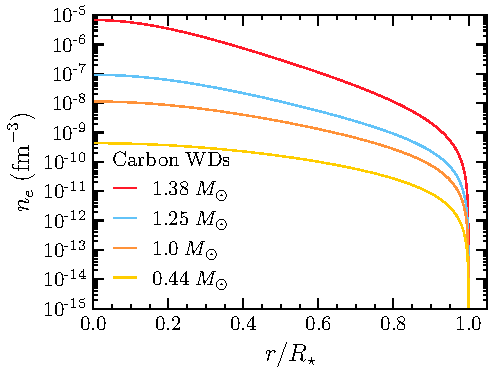
\includegraphics[width = 0.495\textwidth]{ne_prof.pdf}  
    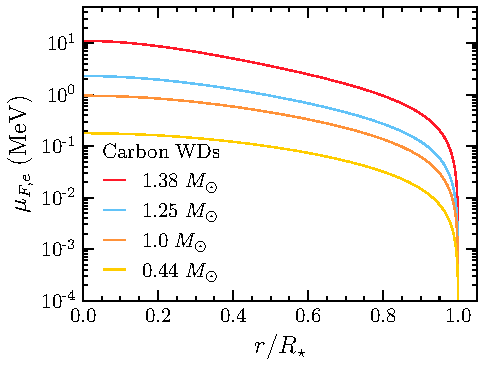
\includegraphics[width = 0.495\textwidth]{muFe_prof.pdf}  
    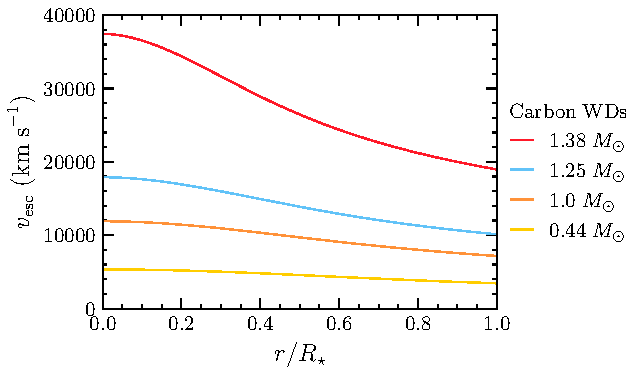
\includegraphics[width = 0.67\textwidth]{vesc_prof.pdf}
    \caption[Electron number density (top left), chemical potential (top right), and escape velocity (bottom) radial profiles for the carbon WDs with FMT EoS in Table~\ref{ch2:tab:WDs}.]{Electron number density (top left), chemical potential (top right), and escape velocity (bottom) radial profiles for the carbon WDs with FMT EoS in Table~\ref{ch2:tab:WDs}. The radial distance of each profile has been normalised to the radius of the star.}
    \label{ch2:fig:WDradprofs}
\end{figure}
%%%%%%%%%%%%%%%%%%%%%%%%%%%%%%%%%%%%%


The mass-radius relations obtained from a zero-temperature EoS begin to deviate from observations for low-mass WDs. 
To address this discrepancy, finite temperature effects can be introduced to the EoS~\cite{deCarvalho:2013rea_Relativisticfeynmanmetropolistellertreatment}. 
The extension to finite temperatures is made by reintroducing the temperature dependence in the Fermi-Dirac
distributions. Now, the electron chemical potential is no longer simply the Fermi energy of the system due to thermal corrections. Define the finite temperature Fermi-Dirac integrals of degree $s$ as
\begin{equation}
    F_s (\eta, \beta) = \int_0^\infty \frac{t^s\sqrt{1 + (\beta/2)t}}{1 + e^{t - \eta}}dt,
\end{equation}
where we define the dimensionless quantities 
\begin{align}
    t & = \frac{E_e - m_e}{\Tstar},\\
    \eta & = \frac{\varepsilon_{F,e}}{\Tstar},\\
    \beta & = \frac{\Tstar}{m_e},
\end{align}
for a star at temperature $\Tstar$. The Thomas-Fermi equilibrium condition within the WS cell is now given by 
\begin{equation}
    \varepsilon_{F,e}(r) - e V(r) = \Tstar \eta(r) - e V(r) = \mathrm{constant},
\end{equation}
with the Coulpmb potential vanishing at the boundary of the cell as before. We now make the change of variables into the dimensionless quantities $\chi/r = \varepsilon_{F,e} / (\hbar c)$ and $x = x/x_\mathrm{WS}$ so that the Poisson equation~\ref{ch2:eq:poisson_WS_cell} becomes
\begin{align}
    \begin{split}
        \frac{d^2 \chi}{dx^2} &= -4 \pi \alpha_\mathrm{EM} x \left( \frac{3}{4\pi \Delta^3} \theta(x_c - x) \right.\\
        &\hspace{7em}\left. - \frac{\sqrt{2}}{\pi^2} \left( \frac{m_e}{m_\pi} \right)^2\left[ F_{1/2}(\eta, \beta) + \beta  F_{3/2}(\eta, \beta) \right] \right),
    \end{split}\\
    \eta(x) & = \left(\frac{1}{\lambda_\pi \Tstar}\right)\frac{\chi(x)}{x},
\end{align}
with the same boundary conditions as in Eq.~\ref{ch2:eq:TF_bc}.

The total energy of the cell remains very similar to the zero-temperature case, with the main differences being that it gains a contribution from the thermal motion of the nucleus, 
\begin{equation}
    E_\mathrm{th} = \frac{3}{2}\Tstar,
\end{equation} 
and that the electron energy density is now given by
\begin{equation}
    \mathcal{E}_e = m_e n_e + \frac{\sqrt{2}}{\pi^2} m_e^4 \beta^{5/2} \left[ F_{3/2}(\eta, \beta) + \beta F_{5/2}(\eta, \beta) \right].
\end{equation}

The pressure of the cell will now gain contributions from the motion of the nucleus as well as the electron, such that the total pressure is
\begin{align}
    P_\mathrm{tot} & = P_N + P_e,\\
    P_N & = \frac{2}{3}\frac{E_\mathrm{th}}{V_\mathrm{WS}} = \frac{\Tstar}{V_\mathrm{WS}},\\
    P_e & = \frac{2^{3/2}}{3\pi} me^4 \beta^{5/2}\left[  F_{3/2}(\eta(x_\mathrm{WS}), \beta) + \beta F_{5/2}(\eta(x_\mathrm{WS}), \beta)  \right].
\end{align}

In Fig.~\ref{ch2:fig:WD_mass_radius} we show the Mass-Radius relations obtained from the zero temperature FMT EoS together with several finite temperature configurations. As can be seen, the deviations from the zero temperature approximation begin at rather high temperatures, $\Tstar\gtrsim 10^7\K$, for masses $\lesssim 0.6 \Msun$. Additionally, we show a random selection of 20,000 WDs presented in the Gaia early data release 2 (EDR2) report~\cite{GentileFusillo_feb_GaiaDataRelease} as the yellow-red dots. The colour of the dot represents the internal temperature of the corresponding WD. The core temperature must be determined from the observed effective surface temperature of the star\footnote{The effective temperature is the temperature that characterises the surface of the star. Assuming that WDs are perfect blackbody emitters, the luminosity will be $L_\gamma = 4\pi \sigma_{SB} \, \Rstar^2 \, \Teff^4$, where $\sigma_{SB}$ is the Stefan–Boltzmann constant.}, with the relation between the two depending on the composition of the WD atmosphere. To obtain the central temperature from the reported effective temperatures, we use the WD cooling sequences generated in Ref.~\cite{Bedard_oct_Spectralevolutionhot}\footnote{The cooling sequence data can be obtained from \url{http://www.astro.umontreal.ca/~bergeron/CoolingModels}} assuming a thin hydrogen atmosphere. In general, there is good agreement between the mass-radius relations derived from the finite temperature FMT EoS and the observed internal temperatures of the WDs.

Given the non-linear nature of the differential equations that describe the FMT EoS (both at zero and finite temperatures), solving the system is a numerically challenging task. As there are no publically available resources to help solve these systems, a significant amount of time was put into solving this problem. The system is solved numerically using the non-linear shooting technique.

\begin{figure}[t!bp]
    \centering
    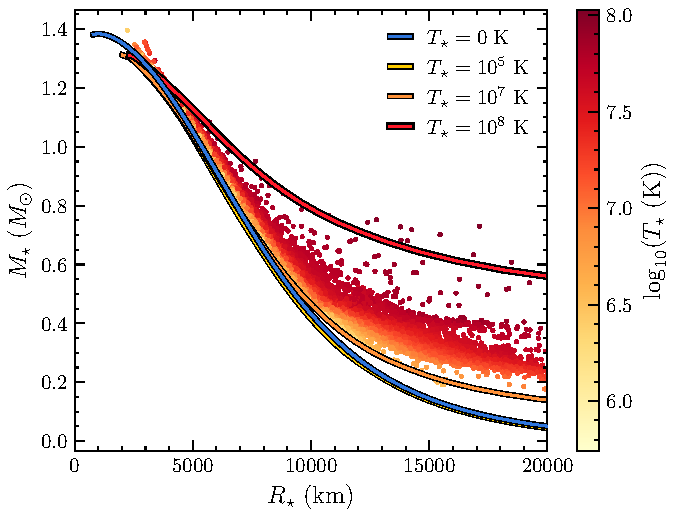
\includegraphics{WD_mass_radius.pdf}
    \caption[Mass-Radius relation of WDs calculated from the FMT EoS in the zero-temperature approximation (dark blue), at $10^{5}\K$ (yellow), $10^{7}\K$ (orange), and $10^{8}\K$ (red), together with observed WDs from Gaia EDR2 observations~\cite{GentileFusillo_feb_GaiaDataRelease} (yellow-red dots).]{Mass-Radius relation of WDs calculated from the FMT EoS in the zero-temperature approximation (dark blue), at $10^{5}\K$ (yellow), $10^{7}\K$ (orange), and $10^{8}\K$ (red), together with observed WDs from Gaia EDR2 observations~\cite{GentileFusillo_feb_GaiaDataRelease} (yellow-red dots). The colour of the dots represents the surface temperature of the WD inferred from cooling models~\cite{Bedard_oct_Spectralevolutionhot}.}
    \label{ch2:fig:WD_mass_radius}
\end{figure}
%%%%%%%%%%%%%%%%%%%%%%%%%%%%%%%%%%%%%


%%%%%%%%%%%%%%%%%%%%%%%%%%%%%%%%%%%%%
%%%%%%%%%%%%%%%%%%%%%%%%%%%%%%%%%%%%%
\subsection{Observational Status}
\label{ch2:subsec:WD_obs}
%%%%%%%%%%%%%%%%%%%%%%%%%%%%%%%%%%%%%
%%%%%%%%%%%%%%%%%%%%%%%%%%%%%%%%%%%%%

The rate at which the energy of the WD core is radiated away is determined by the outer non-degenerate layers of the atmosphere. 
Spectroscopic observations shed light on the composition of these layers and can be used to classify WDs in terms of $\sim$ six spectral types. 
Most of the observed WDs lie in the DA (hydrogen-rich) and DB (helium-rich) categories.  Note that as WDs slowly cool, they undergo spectral evolution. There is a well-defined relation between their luminosity and age (cooling time) that, together with recent breakthroughs in theory and observations, allow us to estimate the age of the stars within the solar neighbourhood and to date the nearest star clusters~\cite{Hansen:2004ih_HSTobservationswhite,Hansen:2007ve_Whitedwarfcooling,Bedin:2009it_jun_Endwhitedwarf,Hansen:2013gda_aug_Agedifferencetwo,Kilic_mar_Agesthindisk}. 

Over the past few decades, WDs have been extensively observed using photometry and spectroscopy. Most of the WDs have been discovered by large area surveys, such as the Sloan Digital Sky Survey (SDSS)~\cite{SDSS:2000hjo_Sloandigitalsky}. However, these local samples are dominated by young WDs with relatively high effective temperatures ($\Teff\gtrsim10^4\K$)~\cite{SDSS:2006iiz_Catalogspectroscopicallyconfirmed,Kleinman:2012nt_jan_SDSSDR7white,Tremblay_sep_Fieldwhitedwarf,Kepler_mar_Whitedwarfmass,Kepler_jun_Whitedwarfsubdwarf}. 
Recently, the local volume sample of nearby stars within $\sim100\pc$ has been catalogued by the Gaia spacecraft~\cite{Gaia:2018vmj_aug_Gaiadatarelease,Gaia:2020wqu_may_Gaiaearlydata}, an astrometric mission. New WD candidates have been identified~\cite{GentileFusillo_feb_GaiaDataRelease}, followed by dedicated spectroscopic observations~\cite{Tremblay_jul_Gaiawhitedwarfs,McCleery_jul_Gaiawhitedwarfs}, increasing the local sample of cool WDs ($\Teff\lesssim5000\K$). 

On the other hand, globular clusters (GCs) are the oldest known stellar systems in the Galaxy. Among them is Messier 4 (M4), also classified as NGC 6121, which is the closest globular cluster to Earth being $\sim 1.9\kpc$ away ~\cite{Neeley_jul_Distanceglobularcluster,Watkins_apr_Tychogaiaastrometricsolution,Shao_nov_GaiaparallaxMilky}. 
The age of M4, $11.6\Gyr$, has been estimated using observations of faint cold WDs with the Hubble Space Telescope  (HST)~\cite{Hansen:2004ih_HSTobservationswhite,Bedin:2009it_jun_Endwhitedwarf}. 
This HST data, corrected for reddening and extinction, 
was converted into luminosities and effective temperatures in ref.~\cite{McCullough:2010ai_CaptureInelasticDark}. From these calculations, it is possible to infer WD radii and their corresponding masses by assuming a mass-radius relation. 

% We should note that there is no evidence so far that globular clusters are embedded in DM halos. Furthermore, there is no consensus on the scenario that leads to globular cluster formation. Observations and simulations suggest that there is more than one plausible mechanism. In the hierarchical structure formation scenario of standard cosmology, old, metal-poor, globular clusters are formed within their halos before or shortly after the onset of reionization~\cite{Peebles:1984zz_feb_Darkmatterorigin,Bromm:2002jt_Formationfirstglobular,Mashchenko:2004hj_Globularclustersdark,Mashchenko:2004hk_Globularclustersdark,Ricotti:2016zhz_Commonoriginglobular}. Old globular clusters with intermediate metallicities, such as M4~\cite{Carretta:2009cn_oct_NaOanticorrelationHB,Carretta:2009cq_oct_NaOanticorrelationHB,Wang_nov_SodiumabundancesAGB}, could have been accreted from small satellite galaxies and lost a large fraction of their initial DM content due to tidal stripping by the host galaxy~\cite{Bromm:2002jt_Formationfirstglobular,Mashchenko:2004hk_Globularclustersdark,Saitoh:2005tt_Tidaldisruptiondark}, though a small DM fraction could have survived in the innermost region of the cluster~\cite{Mashchenko:2004hk_Globularclustersdark,Ibata:2012eq_Globularclusterspossess}. 
% Since the cool WDs observed in M4 are located in the dense core of the globular cluster, well within the tidal radius, it is expected that the DM content in this region has survived tidal disruption. Under this assumption, it is possible to estimate the DM density as outlined in refs.~\cite{Bertone:2007ae_CompactStarsDark,McCullough:2010ai_CaptureInelasticDark}.  The DM density at the largest radius the WDs were observed ($2.3 \pc$) was conservatively estimated to be $\rho_\chi =798~(531.5) \GeV\cm^{-3}$  for a contracted (uncontracted) NFW profile \cite{McCullough:2010ai_CaptureInelasticDark}. 
% It is worth noting that the DM density in M4 was found to be of the order of few $\GeV/\cm^3$ in ref.~\cite{Hooper:2010es_InelasticDarkMatter}. However, the estimation in ref.~\cite{McCullough:2010ai_CaptureInelasticDark} for M4, adopted in this work, is in good agreement with that of ref.~\cite{Amaro-Seoane:2015uny_jun_Probingdarkmatter} for the GC Omega Centauri (NGC 5139).



%%%%%%%%%%%%%%%%%%%%%%%%%%%%%%%%%%%%%
%%%%%%%%%%%%%%%%%%%%%%%%%%%%%%%%%%%%%
%%%%%%%%%%%%%%%%%%%%%%%%%%%%%%%%%%%%%
\section{Neutron Stars}
\label{ch2:sec:neutron_stars}
%%%%%%%%%%%%%%%%%%%%%%%%%%%%%%%%%%%%%
%%%%%%%%%%%%%%%%%%%%%%%%%%%%%%%%%%%%%
%%%%%%%%%%%%%%%%%%%%%%%%%%%%%%%%%%%%%

Being the end product of massive, $\gtrsim 8 \Msun$, stars, there are significantly fewer NSs than the WDs discussed above. As their name suggests, they are composed primarily of neutrons, which provide the degeneracy pressure required to prevent the gravitational collapse of the star.
The internal structure of an NS is significantly more complicated than that of a WD. Broadly speaking, an NS can be divided into five main regions. We give an overview of the important features of each of these regions, and point the reader to Refs.~\cite{Glendenning_Compactstarsnuclear, Lattimer:2004pg_Physicsneutronstars, Haensel_NeutronstarsEqation, Weber:2007ch_may_NeutronStarInteriors, Camenzind_Compactobjectsastrophysics, Ozel:2015fia_Densematterequation,Ozel:2016oaf_jul_MassesRadiiEquation,Lattimer:2021emm_jul_NeutronStarsNuclear} for more indepth discussions. Working from the outside in, these regions are:

\subsubsection*{Atmosphere}
The atmosphere is an extremely thin layer of plasma that makes up less than 1\% of the NS mass. However, it plays an extremely important role as the observed spectrum radiation emitted by the star must pass through this region~\cite{Lattimer:2004pg_Physicsneutronstars, Haensel_NeutronstarsEqation}.

\subsubsection*{Outer Crust}
The outer crust is the thin layer of ionized Iron-56 nuclei that extends down until the density reaches the neutron drip point, $\rho_\star = \rho_\mathrm{ND} \sim 4.3\times 10^{11}\g\cm^{-3}$. This is the density at which neutrons begin to drip from the nuclei as their chemical potentials approach zero. The ionized electrons form a non-relativistic but degenerate gas, with their chemical potentials increasing as the density increases. This leads to the ``neutronisation'' of the nuclei as the beta-capture of electrons by protons increases.

\subsubsection*{Inner Crust}
The density within the inner crust spans the range between $\rho_\mathrm{ND}\lesssim \rho_\star \lesssim 0.5\rho_0$, with $\rho_0 \sim 2.8\times 10^{14}\g\cm^{-3}$ the nuclear saturation density (i.e. the density of nuclear matter)~\cite{Lattimer:2004pg_Physicsneutronstars,Haensel_NeutronstarsEqation,Grill:2014aea_Equationstatethickness}. Here, the neutrons that have dripped from the nuclei will potentially form a superfluid. Towards the crust-core boundary, the nuclear lattice begins taking on interesting topological structures that are distinguished by the configuration of the voids in the lattice. These are known as the so-called \textit{pasta phases}~\cite{Watanabe:2004tr_SimulationtransitionsPasta,Avancini:2010ch_Warmpastaphase,Yakovlev:2015vma_Electrontransportnuclear} of nuclear matter, which include 2D sheets (lasagna), cylindrical rods (spaghetti), or 3D clumps (gnochi).
% \begin{itemize}
%     \item 2D void cylinders creating spaghetti structures of nuclei
%     \item Planar voids with slabs of nuclei forming lasagna sheets
%     \item 3D cylindrical voids leading to thin 2D cylinders of nuclear ziti
%     \item 3D spherical voids enclosed by ravioli
%     \item 2D circular voids in sheets of Swiss cheese
% \end{itemize}
Eventually, towards the crust-core interface the nuclear matter transitions into a uniform medium\footnote{The nuclear minestrone, if you will.}. 

\subsubsection*{Outer Core}
Once densities go above $0.5\rho_0$, the nuclear clusters will dissolve into a homogenous fluid that is composed of neutrons, protons, electrons, and muons known as $npeu$ matter. The relative abundances of the species, $Y_i=n_i/n_b$, are dictated by the conditions of electrical neutrality and beta-equilibrium.
Charge neutrality dictates that the abundances of the charged particles obeys
\begin{equation}
    Y_p = Y_e + Y_\mu,
\end{equation}
while beta-equilibrium refers to the balance between the weak decays of neutrons and the electron/muon capture by the protons,
\begin{gather}
    n \rightarrow p + \ell^- +\bar{\nu}_\ell,\label{ch2:eq:beta_decay}\\
    p + \ell^- \rightarrow n + \nu_\ell,\label{ch2:eq:electron_capture}
\end{gather}
with $\ell = e, \mu$. Muons will begin to replace electrons in these reactions once the electron chemical potential exceeds the mass of the muon, $\mu_{F,e} \gtrsim m_\mu = 105.7\MeV$. As neutrinos are assumed to escape the NS once produced, the relation between the chemical potential of the leptons is simply
\begin{equation}
    \mu_{F,e} = \mu_{F,\mu}.
\end{equation}
The outer core region ends once the density reaches $\rho_\star \sim 2\rho_0$, and we transition into the inner core.

\subsubsection*{Inner Core}
The densities within the inner cores of NSs extend between $2\rho_0 \lesssim \rho_\star \lesssim (10-15)\rho_0$ and are hence a mystery to this day. As the density greatly exceeds any material that can be produced in a laboratory, the exact composition of this region is unknown and depends on the equation of state one adopts to describe it. Some of the more well-known candidates are
\begin{itemize}
    \item A hyperonic  matter component, i.e. nucleons containing a valence strange quark. These appear once the neutron chemical potential equals that of the $\Lambda^0$ hyperon, with the $\Xi^-$ appearing once its chemical potential equals the sum of the chemical potentials of the neutrons and electrons~\cite{Weber:2007ch_may_NeutronStarInteriors,Fortin:2014mya_Neutronstarshyperon}. 
    \item Pion/Kaon condensates. These are Bose-Einstein condensates of pion/kaon-like excitations~\cite{Baym:1973zk_Pioncondensationnuclear,Baym:1974vzp_Pioncondensationneutron,Kaplan:1986yq_StrangeGoingsDense, Ellis:1995kz_Kaoncondensationneutron, Brown:1992ib_Novelmechanismkaon, Ma:2022fmu_jan_Kaonmesoncondensate}. 
    \item A quark-gluon plasma comprised of deconfined $u,\; d$ and $s$ quarks and gluons~\cite{Akmal:1998cf_Equationstatenucleon,Baym:2006rq_Neutronstarsquark,Baym:2017whm_Hadronsquarksneutron}.
\end{itemize}


%%%%%%%%%%%%%%%%%%%%%%%%%%%%%%%%%%%%%
%%%%%%%%%%%%%%%%%%%%%%%%%%%%%%%%%%%%%
\subsection{Observational Status}
\label{ch2:subsec:NS_obs}
%%%%%%%%%%%%%%%%%%%%%%%%%%%%%%%%%%%%%
%%%%%%%%%%%%%%%%%%%%%%%%%%%%%%%%%%%%%

Unlike the WDs discussed above, there are significantly fewer NS observations to constrain the EoS. However, recent years have seen significant strides in furthering our understanding of matter at super-nuclear densities, both from a theory and observational standpoint. On the theoretical side, these advances come from developments in chiral EFT allowing more detailed modelling of nuclear interactions~\cite{Hebeler:2009iv_Chiralthreenucleonforces, Tews:2012fj_jan_NeutronMatterNexttoNexttoNexttoLeading, Tews:2018kmu_jun_Constrainingspeedsound}. The observational data has been bolstered thanks to the onset of gravitational wave astronomy due to the LIGO-VIRGO experiment~\cite{LIGOScientific:2017zic_Gravitationalwavesgammarays, LIGOScientific:2018cki_oct_GW170817MeasurementsNeutron, LIGOScientific:2018hze_Propertiesbinaryneutron} and the launch of the Neutron star Interior Composition Explorer (NICER) X-ray timing instrument. 

Ultimately, what is needed to further constrain the NS EoS are more precise observations of NS masses and radii, which can be obtained from various observational techniques. NS masses have historically been much easier to measure than their radii. In particular, masses of NSs in binary systems can be precisely determined as the underlying gravitational theories are well-understood today~\cite{Steiner:2010fz_Equationstateobserved, Lattimer:2013hma_Neutronstarmasses, Ozel:2015fia_Densematterequation,Ozel:2016oaf_jul_MassesRadiiEquation, Miller:2016pom_Observationalconstraintsneutron}. The radii must be determined by assuming the NSs emit a blackbody spectrum, however, this method is only reliable for cool NSs where the atmospheric models are well understood~\cite{Miller:2016pom_Observationalconstraintsneutron}. 

The NICER experiment can provide much more precise measurements of NS radii than previous methods. This is achieved ny measuring the X-ray pulse profiles of pulsars, that are sensitive to how light bends around the star. This provides information on the compactness of the star, $G M_\star/R_\star c^2$, that can be used to determine $M_\star$ and $R_\star$ given that the mass can usually be determined through other means. The heaviest NS observed to date, the millisecond pulsar PSR J0740+6620~\cite{Miller:2021qha_sep_RadiusPSRJ0740, Riley:2021pdl_sep_NICERViewMassive}, had its mass determined by measuring the relativistic Shapiro time delay~\cite{Shapiro:1964uw_FourthTestGeneral}\footnote{This refers to the time it takes for light to move out of a gravitational well taking longer than the naive Newtonian prediction due to the curvature of space-time.} of the radio signal, allowing the radius to be obtained once the compactness was measured~\cite{NANOGrav:2019jur_sep_RelativisticShapirodelay}. Refined analyses result in a mass of 2.08$\pm$0.07$\Msun$~\cite{Fonseca:2021wxt_jul_RefinedMassGeometric} and a radius of $12.39^{+1.30}_{-0.98} \km$~\cite{Riley:2021pdl_sep_NICERViewMassive} or $13.71^{+2.61}_{-1.50} \km$~\cite{Miller:2021qha_sep_RadiusPSRJ0740} at 68\% confidence levels. 


Gravitational wave astronomy offers an alternative and independent determination of NS masses and radii to the electromagnetic observations above. The best candidate events for this analysis are NS binary mergers, though these are expected to be an uncommon occurrence. As the NSs inspiral toward each other, they will begin to deform due to the tidal forces they induce on one another~\cite{Lattimer:2019eez_jun_NeutronStarMass}. 
This deformation will alter the waveform observed at the detectors, with the shift in the phase of the waveform depending on the mass ratio, $q = M_2/M_1 <1$, the chirp mass of the system, $\mathcal{M}_\mathrm{chirp} = (M_1 M_2)^{3/5}/(M_1 + M_2)^{1/5}$, and a combination of the tidal deformabilities, $\tilde\Lambda$. The latter refers to how susceptible the star is to deformation due to tidal forces acting upon it, with larger values corresponding to less compact objects. Comparing the observed waveform to that determined from precise numerical simulations allows constraints to be placed on these parameters, and ultimately on the masses and radii of the merging NSs.

Furthermore, the electromagnetic emission from the remnant object provides information about the maximum mass an NS can achieve. 
If the mass of the remnant object is too large, it will collapse into a black hole, and it is highly unlikely that a gamma-ray burst will occur. If the remnant does not immediately collapse, then its mass and how it is rotating determines whether it will be hydrodynamically stable, unstable, or metastable against gravitational collapse. A remnant that undergoes differential rotation\footnote{This is when components of the star at different latitudes have different angular velocities.} can support heavier masses than one that is uniformly rotating. Hence, the afterglow spectrum can inform us as to how the star is rotating. Comparing the maximum mass supported by this rotation to the initial mass after inspiral yields an upper bound on the maximum NS mass achievable. 

To date, the only confirmed NS-NS merger is the merger event GW170817 observed at LIGO-VIRGO in 2017~\cite{LIGOScientific:2018cki_oct_GW170817MeasurementsNeutron,LIGOScientific:2018hze_Propertiesbinaryneutron}, with the gamma-ray burst counterpart signal observed at the Fermi Gamma-ray Burst Monitor and INTEGRAL satellite~\cite{LIGOScientific:2017zic_Gravitationalwavesgammarays}. These observations led to the constraint that the radius of a $1.4\Msun$ NS has an upper bound of $R_{1.4} < 13.3\km$~\cite{LIGOScientific:2018cki_oct_GW170817MeasurementsNeutron, De:2018uhw_aug_TidalDeformabilitiesRadii}, and that the maximum NS mass must be $M_\mathrm{NS}^\mathrm{MAX} < 2.18\Msun$~\cite{LIGOScientific:2017zic_Gravitationalwavesgammarays}. These constraints on the neutron star mass-radius relation are shown as the shaded turquoise and red regions of Fig~\ref{ch2:fig:NS_mass_rad}. 

%%%%%%%%%%%%%%%%%%%%%%%%%%%%%%%%%%%%%
\begin{figure}[t!bp]
    \centering
    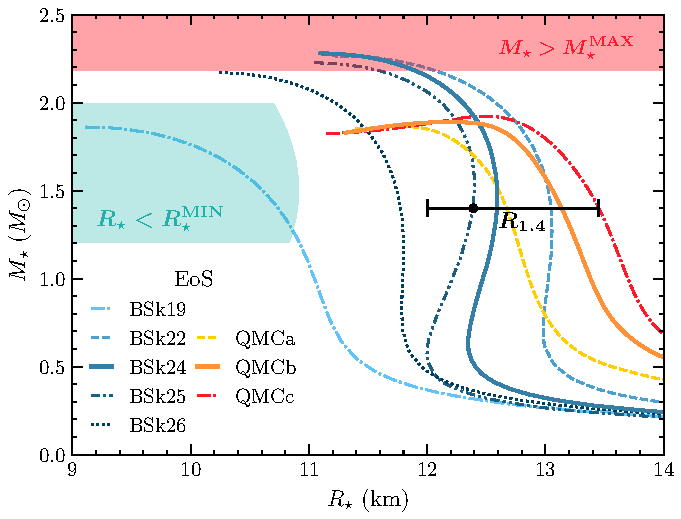
\includegraphics{NS_mass_radius.pdf}
    \caption[Neutron Star Mass-Radius relation predicted by the BSk (blue lines) and QMC (red lines) EoSs.]{Neutron Star Mass-Radius relation predicted by the BSk (blue lines) and QMC (red lines) EoSs. Constraints obtained from the gravitational wave event GW170817 are shown as the shaded regions, with the lower bound on the radius in turquoise, and the maximum NS mass possible in red. The line band labeled $R_{1.4}$ indicates the constraints on the radius of a $1.4\;\Msun$ NS.}
    \label{ch2:fig:NS_mass_rad}
\end{figure}
%%%%%%%%%%%%%%%%%%%%%%%%%%%%%%%%%%%%%



%%%%%%%%%%%%%%%%%%%%%%%%%%%%%%%%%%%%%
%%%%%%%%%%%%%%%%%%%%%%%%%%%%%%%%%%%%%
\subsection{Neutron Star Equations of State}
\label{ch2:subsec:NS_EoS}
%%%%%%%%%%%%%%%%%%%%%%%%%%%%%%%%%%%%%
%%%%%%%%%%%%%%%%%%%%%%%%%%%%%%%%%%%%%

Given the scarce constraints that have been placed on the NS mass-radius relation, there are numerous equations of state in the literature that can be used to incorporate the internal structure into our calculations. In this work, we adopt two different EoSs, which we detail here. 

\subsubsection{The Brussels-Montreal EoS}
The first family of EoSs adopted in this work are based on the Brussels-Montreal (BSk) energy density functionals~\cite{Chamel:2009yx_FurtherexplorationsSkyrmeHartreeFockBogoliubov, Goriely:2010bm_FurtherexplorationsSkyrmeHartreeFockBogoliubov, Pearson:2011zz_jun_Propertiesoutercrust, Pearson:2012hz_Innercrustneutron, Potekhin:2013qqa_Analyticalrepresentationsunified, Pearson:2018tkr_Unifiedequationsstate}, for cold, non-accreting NSs. In these models, the density-dependent nucleon interactions are accounted for via a mean-field approximation in either the Hartree-Fock (HF) or Hartree-Fock-Bogoliubov (HFB) formalism\footnote{The HF method accounts for the energy associated with nucleon pairings, while the HFB method neglects this contribution.}, through effective Skyrme type forces~\cite{Bender:2003jk_Selfconsistentmeanfieldmodels, Stone:2006fn_Skyrmeinteractionfinite}. The BSk EoS family are unified EoSs, meaning they describe all the regions of the NS interior using the single effective Hamiltonian. Furthermore, the authors provide public \texttt{FORTRAN} subroutines that implement fits to the EoS quantities such as the pressure and density as functions of the baryon number density, allowing straightforward implementation of the EoS. 

The authors provide these fits to eight configurations of the BSk EoS, labeled BSK19-26. Of these, the older BSK19-21  functionals were fitted to older atomic mass data that has since been updated in the newer models, BSk22-26. The mass-radius relation predicted by a selection of these models is shown in Fig.~\ref{ch2:fig:NS_mass_rad} by the blue lines. Missing are the BSk20 and 21 models, as they give very similar results to the 26 and 24 models respectively. The BSk19 EoS is partially ruled out from the lower bound on NS radii obtained from the electromagnetic counterpart of the GW170817 event~\cite{Koppel:2019pys_Generalrelativisticdeterminationthreshold}, while BSk22 is ruled out from constraints on the tidal deformability from the same event~\cite{Perot:2019gwl_Rolesymmetryenergy}. Additionally, BSk22 does not support the presence of direct Urca\footnote{This is another name given to the reactions in Eqs.~\ref{ch2:eq:beta_decay},~\ref{ch2:eq:electron_capture}.} processes in NSs described by this EoS. These processes are required to explain observations of a small population of NSs that have cooled to temperatures below those predicted by the ``minimal cooling paradigm''~\cite{Gusakov:2004se_Enhancedcoolingneutron, Page:2004fy_MinimalCoolingNeutron}. On the other hand, the BSk26 functional predicts that all stable NSs will support direct Urac processes. This goes against the current observational evidence that a majority of NSs are well modeled by the minimal cooling paradigm, ruling the EoS out. Of the remaining two models, BSk24 and 25, we choose to adopt BSk24 as it gives slightly better fits to NS mass data than that of BSk25. 

We use the BSk24 EoS to generate four benchmark NSs with masses of $1$, 1.5, 1.9 an 2.16$\;\Msun$, with the central density $\rho_c$, stellar mass, radius, metric factor $B(\Rstar)$ and central speed of sound $c_s(0)$ in Table~\ref{ch2:tab:BSk_configs}. 
Radial profiles of the baryon number density $n_b(r)$, metric factor $B(r)$, neutron chemical potential $\kinFn(r)$, and neutron abundance  $Y_n(r)$, are shown in Fig.~\ref{ch2:fig:BSk_profiles}. 



%%%%%%%%%%%%%%%%%%%%%%%%%%%%%%%%%%%%%%%%
\begin{table}[tb]
    \centering
    \begin{tabular}{l c c c c}
    \toprule
     EoS &  BSk24-1 &  BSk24-2 &  BSk24-3 &  BSk24-4 \\ \midrule\midrule
    $\rho_c$ $[\rm{g \, cm^{-3}}]$ & $5.94 \times 10^{14}$   & $7.76 \times 10^{14}$ & $1.04 \times 10^{15}$ & $1.42 \times 10^{15}$  \\
    $\Mstar$ $[\Msun]$ & 1.000 & 1.500 & 1.900 & 2.160  \\
    $\Rstar$ [km] & 12.215  & 12.593 & 12.419 & 11.965 \\
    $B(\Rstar)$ & 0.763 & 0.648 & 0.548 & 0.467\\
    $c_s(0)$ $[c]$ & 0.511 & 0.628 & 0.734 & 0.835 \\
    \bottomrule
    \end{tabular} 
    \caption[Benchmark NSs, for four different configurations of the equations of state (EoS) for cold non-accreting neutron stars with Brussels–Montreal functionals BSk24 \cite{Pearson:2018tkr_Unifiedequationsstate}.]{Benchmark NSs, for four different configurations of the equations of state (EoS) for cold non-accreting neutron stars with Brussels–Montreal functionals BSk24 \cite{Pearson:2018tkr_Unifiedequationsstate}. EoS configurations are determined by the central mass-energy density $\rho_c$.}
    \label{ch2:tab:BSk_configs}
\end{table} 
%%%%%%%%%%%%%%%%%%%%%%%%%%%%%%%%%%%%%%%%

%%%%%%%%%%%%%%%%%%%%%%%%%%%%%%%%%%%%%
\begin{figure}[t!bp]
    \centering
    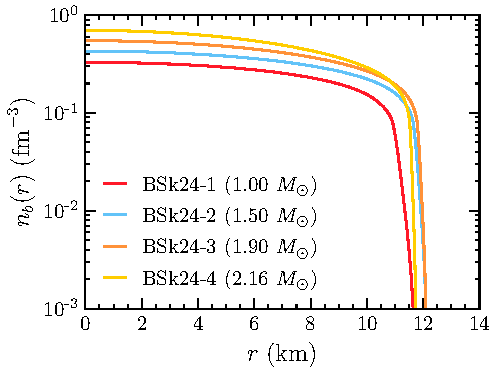
\includegraphics[width=0.495\textwidth]{nb_BSk_prof.pdf}
    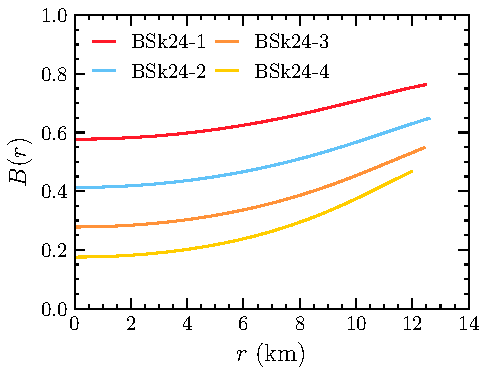
\includegraphics[width=0.495\textwidth]{B_BSk_prof.pdf}
    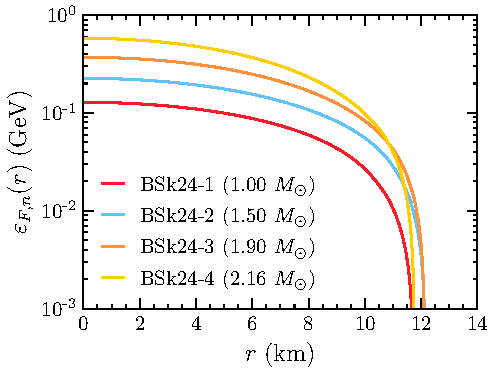
\includegraphics[width=0.495\textwidth]{epsFn_BSk_prof.pdf}
    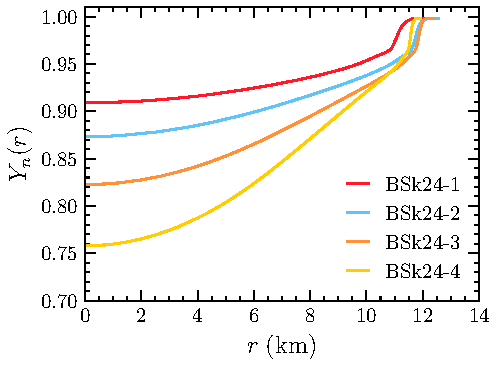
\includegraphics[width=0.495\textwidth]{Yn_BSk_prof.pdf}
    \caption[Radial profiles of the baryon number density (top left), metric factor $B(r)$ (top right), neutron chemical potential (bottom left), and neutron abundance (bottom right) for the four benchmark NS of the BSk24 EoS in Table~\ref{ch2:tab:BSk_configs}.]{Radial profiles of the baryon number density (top left), metric factor $B(r)$ (top right), neutron chemical potential (bottom left), and neutron abundance (bottom right) for the four benchmark NS of the BSk24 EoS in Table~\ref{ch2:tab:BSk_configs}.}
    \label{ch2:fig:BSk_profiles}
\end{figure}
%%%%%%%%%%%%%%%%%%%%%%%%%%%%%%%%%%%%%
    

While BSk24 and 25 lie well within current observational constraints, they are minimal models in that they only account for $npe\mu$ matter, and do not incorporate any exotic species within the NS core. This is problematic as it is highly likely that hyperonic matter will appear in the cores of NS heavier than $\sim 1.7\;\Msun$.  Additionally, the Skyrme forces that describe the nuclear interaction are treated non-relativistically, while the nucleons in heavier stars can become semi-relativistic. To address these concerns, later works~\cite{Anzuini:2021lnv_nov_Improvedtreatmentdark, Bell:2023ysh_dec_ThermalizationAnnihilationDark} adopted the Quark-Meson Coupling (QMC) EoS.



\subsubsection*{The Quark-Meson Coupling EoS}

The second EoS adopted is based on the QMC model of Refs.~\cite{Guichon:1987jp_Possiblequarkmechanism,Guichon:1995ue_Rolenucleonstructure, Saito:2005rv_Nucleonhadronstructure,Guichon:2018uew_QuarkMesonCouplingQMC}, in which baryons are described as bags of three valence quarks, with the bags themselves modeled by the MIT bag model~\cite{Chodos:1974pn_Baryonstructurebag}. The interactions among the baryons are described by the exchange of mesons between the valence non-strange quarks and are formulated within a relativistic mean-field Lagrangian. The exchange of the vector mesons acts as an overall shift to the energy of the baryons\footnote{A simple analogy for this is how the force of an electron in an electromagnetic field is due to the exchange of photons, which are vector fields. The total energy of the electron is a shift relative to the free electron energy.}. The scalar mean fields play a significantly more important role, modifying the effective mass of the baryons. The scalar (and also vector) couplings are density-dependent, leading to an effective mass of the baryons that varies throughout the NS. The density dependence of these couplings is equivalent to including repulsive three-body forces between the baryons and arises naturally in the QMC model through the in-medium modification of the baryonic structure~\cite{Guichon:2004xg_Quarkstructurenuclear,Thomas:2021kio_jul_Rolequarksnuclear}. Additional details on the energy density and couplings of the QMC model adopted in this work are given in Appendix~\ref{appendix:QMC_details}.

The mass-radius relation of three different configurations of the QMC EoS, namely three different choices of the isovector coupling constant, are shown as the red lines in Fig.~\ref{ch2:fig:NS_mass_rad}, obtained from Ref.~\cite{Motta:2019tjc_Isovectoreffectsneutron}. Of these, QMCb (orange solid line in Fig.~\ref{ch2:fig:NS_mass_rad}) lies within the constraints on the radius of a $1.4\;\Msun$ NS from GW170817, and can produce an NS of mass $1.908 \pm 0.016\;\Msun$, the currently preferred mass of PSR J1614-2230 obtained by the NANOGrav collaboration~\cite{NANOGrav:2017wvv_apr_NANOGrav11yearData}\footnote{As mentioned above, the current heaviest NS has a mass of $2.08\pm 0.07\Msun$ though the implications of this on the QMC EoS are beyond the scope of this work.}.

The QMCb EoS data was provided by the authors of Ref.~\cite{Motta:2019tjc_Isovectoreffectsneutron} for use in this work and will be referred to as simply the QMC EoS from here on. From this, we calculate the internal structure of four benchmark QMC NSs, similar to the BSk models of Table~\ref{ch2:tab:BSk_configs}, with the central baryon density replacing the central density and the speed of sound omitted. The relevant parameters are shown in Table~\ref{ch2:tab:QMC_configs}. The top four plots in Fig.~\ref{ch2:fig:QMC_profiles} show the radial profiles for the number densities of the neutrons and protons for each configuration on the left, with their effective masses shown on the right. The bottom two plots of the same figure show the number densities for each species within the heaviest star on the left, including leptons in dashed lines, with the effective masses for each of the baryons on the right. The replacement of high-momentum neutrons with low-momentum hyperons is clearly seen in the bottom left plot, as the neutron number density dips towards the centre of the massive star. As the densities are high enough for the charged hyperon $\Xi^-$ to appear, the abundance of leptons decreases due to the requirement of charge neutrality, also seen in this plot. 

%%%%%%%%%%%%%%%%%%%%%%%%%%%%%%%%%%%%%
\begin{table}[t!bp]
    \centering
    \begin{tabular}{l c c c c}
    \toprule
     EoS &  QMC-1 &  QMC-2 &  QMC-3 &  QMC-4 \\ \midrule\midrule
    $n_{\cal B}^c$ $[\fm^{-3}]$ & 0.325 & 0.447 & 0.540 & 0.872\\
    $\Mstar$ $[\Msun]$ & 1.000 & 1.500 & 1.750 & 1.900  \\
    $\Rstar$ [km] &  13.044 & 12.847 & 12.611 & 12.109 \\
    $B(\Rstar)$ & 0.772 & 0.653 & 0.588 & 0.535\\
    \bottomrule
    \end{tabular} 
    \caption[Benchmark NSs for four different configurations of the QMC equation of state.]{Benchmark NSs for four different configurations of the QMC equation of state. 
    EoS configurations are determined by the central number density $n_{\cal B}^c$.
    }
    \label{ch2:tab:QMC_configs}
\end{table} 
%%%%%%%%%%%%%%%%%%%%%%%%%%%%%%%%%%%%%

%%%%%%%%%%%%%%%%%%%%%%%%%%%%%%%%%%%%%
\begin{figure}[t!bp]
    \centering
    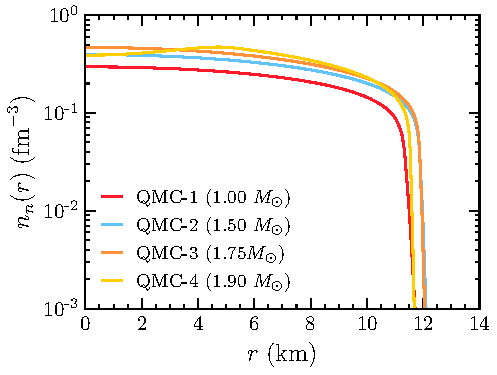
\includegraphics[width=0.495\textwidth]{nn_QMC_profs.pdf}
    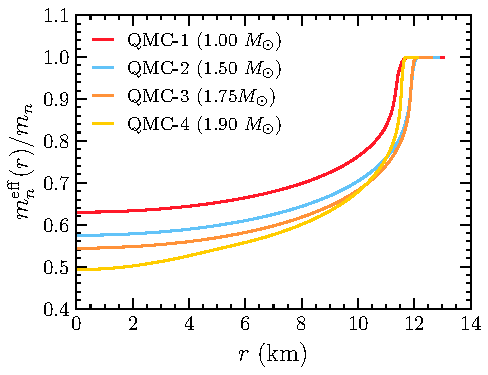
\includegraphics[width=0.495\textwidth]{meff_n_QMC_profs.pdf}
    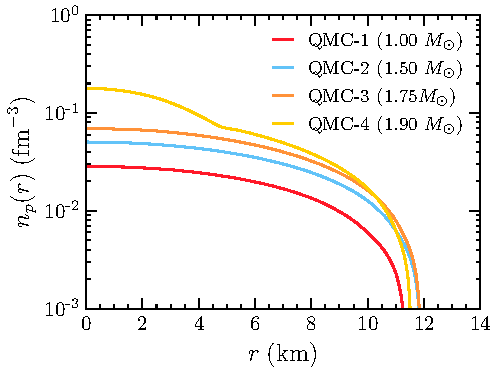
\includegraphics[width=0.495\textwidth]{np_QMC_profs.pdf}
    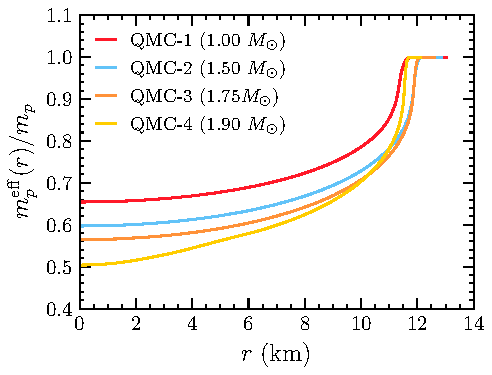
\includegraphics[width=0.495\textwidth]{meff_p_QMC_profs.pdf}
    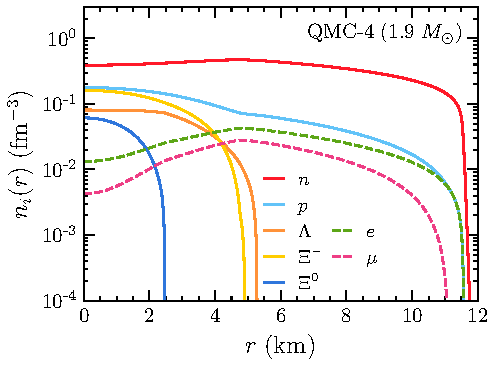
\includegraphics[width=0.495\textwidth]{ni_QMC_profs.pdf}
    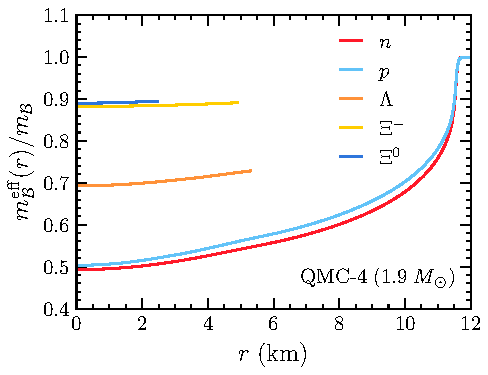
\includegraphics[width=0.495\textwidth]{meff_B_QMC_profs.pdf}
    \caption[Number density profiles (left) and the ratio of the effective mass to the bare mass (right) for neutrons (top) and protons (middle) for benchmark configurations of the QMC EoS in Table~\ref{ch2:tab:QMC_configs}.]{Number density profiles (left) and the ratio of the effective mass to the bare mass (right) for neutrons (top) and protons (middle) for benchmark configurations of the QMC EoS in Table~\ref{ch2:tab:QMC_configs}. In the bottom panels, we show the same profiles for all species in the heaviest NS considered, QMC-4, which contains hyperonic matter.}
    \label{ch2:fig:QMC_profiles}
\end{figure}
%%%%%%%%%%%%%%%%%%%%%%%%%%%%%%%%%%%%%
